\subsection{Interfaccia}\label{interfaccia}
In questa sezione viene riportata una spiegazione dettagliata dell'interfaccia con la libreria utilizzata per la sua realizzazione, le sue componenti e il suo funzionamento.
\subsubsection{PySide2}\label{pyside2}
Per la realizzazione dell'interfaccia è stata utilizzata la libreria \emph{PySide2}, prodotto del progetto \emph{Qt for Python} che ha l'obiettivo di fornire il completo supporto e porting del modulo \emph{Qt 5} in \emph{C++}.\\
La libreria offre un framework per lo sviluppo di interfacce utente con design di alto livello per la realizzazione di applicazioni di alta qualità.\\
La documentazione della libreria è ben aggiornata e dettagliata con casi d'uso ed esempi. La facilità è aumentata dal fatto di avere la stessa sintassi e semantica di \emph{Qt} per \emph{C++} quindi, per chi proviene da questa piattaforma, l'uso è praticamente immediato.

\subsubsection{Componenti Interfaccia} \label{compInterfaccia}
L'interfaccia (Figura \ref{fig:interfaccia}) comprende tre componenti principali. Il componente principale \emph{MainWindow} che a sua volta ne contiene altri due: \emph{Toolbar} e \emph{Content}.

\begin{figure}[H]
    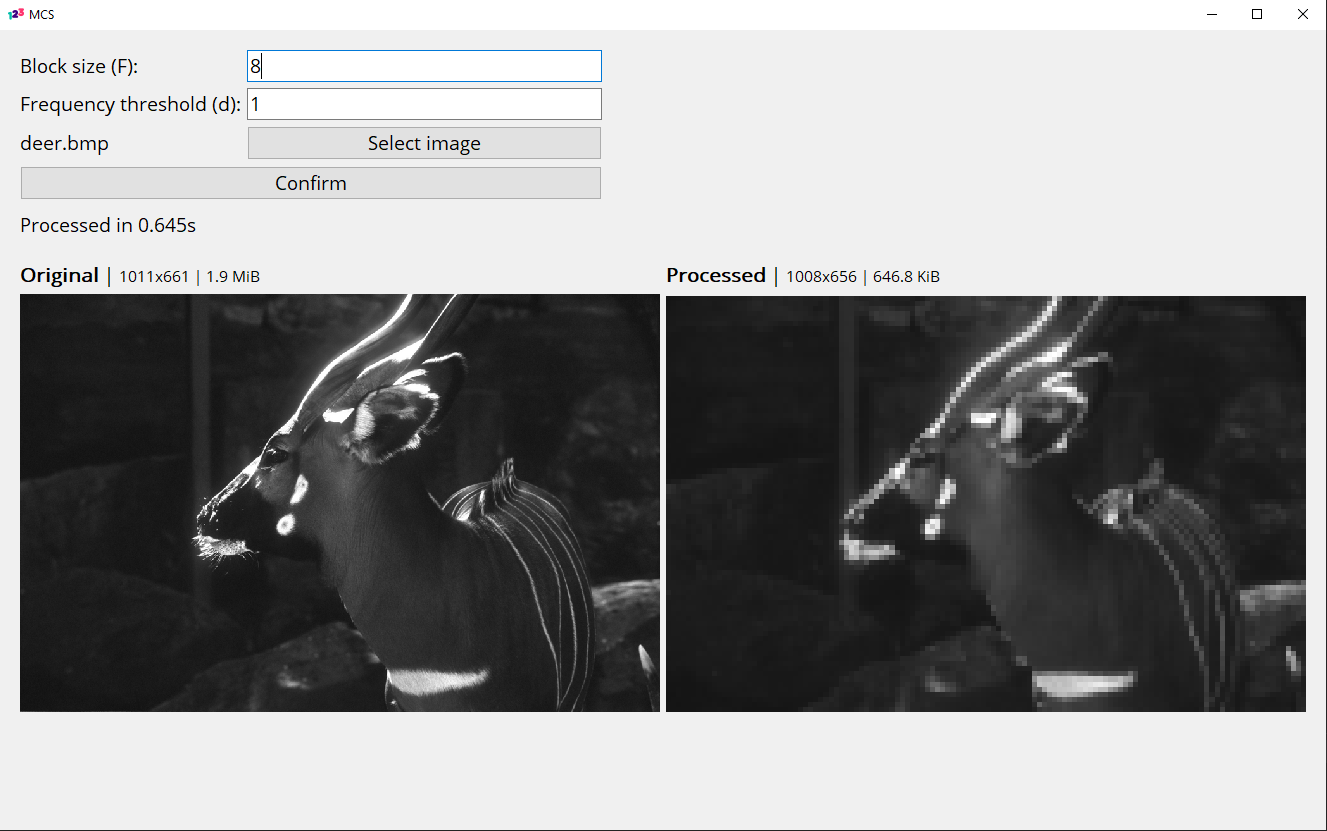
\includegraphics[scale=0.3]{gui}\centering
    \caption{Interfaccia utente}\label{fig:interfaccia}
\end{figure}

La \textbf{Toolbar} è il 'core' dell'interfaccia; contiene un form per inserire i campi che fanno riferimento alle variabili F (Block Size) e d (Fequency Threshold). Inoltre è presente un bottone per la selezione di un'immagine dal filesystem in formato \emph{bmp} con la label corrispondente al nome dell'immagine selezionata.\\
È importante sottolineare che grazie all'utilizzo della libreria \emph{OpenCv} è possibile leggere un'immagine in scala di grigi in cui ogni pixel è costituito da un byte che può assumere valori compresi tra 0 e 255. Se non specificato diversamente, i valori dei pixels vengono convertiti alla profondità di 8 bit\footnote{\url{https://docs.opencv.org/3.4/d4/da8/group__imgcodecs.html}}.
Infine è presente un bottone \emph{Confirm} per eseguire l'algoritmo di compressione dell'immagine in base ai parametri scelti: premendolo, se i parametri sono validi, una progressbar mostra l'avanzamento dell'algoritmo e al suo termine viene riportato il tempo impiegato per il completamento.\\
Il processo di compressione dell'immagine e aggiornamento della barra di caricamento avviene in un thread di lavoro differente dal thread principale per evitare il \emph{freeze} dell'interfaccia utente.\\
In figura \ref{fig:toolbarloading} e in figura \ref{fig:toolbardone} vengono mostrate rispettivamente la toolbar durante l'esecuzione dell'algoritmo di compressione e una volta terminata la computazione.

\begin{figure}[H]
    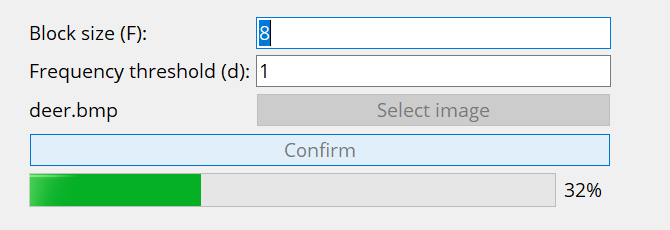
\includegraphics[scale=0.5]{toolbar-loading}\centering
    \caption{Toolbar durante l'esecuzione dell'algoritmo di compressione}\label{fig:toolbar loading}\label{fig:toolbarloading}
\end{figure}
\begin{figure}[H]
    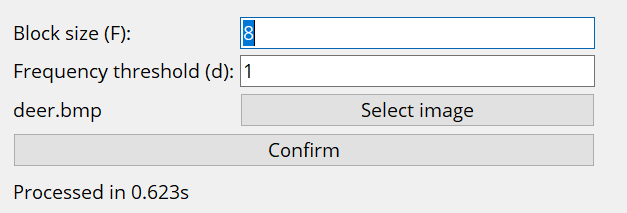
\includegraphics[scale=0.54]{toolbar-done}\centering
    \caption{Toolbar che mostra il tempo impiegato dall'algoritmo di compressione}\label{fig:toolbardone}\label{fig:toolbardone}
\end{figure}

Il componente \textbf{Content} si occupa di visualizzare l'immagine originale selezionata dal filesystem e la stessa una volta compressa.
Vengono inoltre riportate alcune misure tra cui le dimensioni dell'immagine e lo spazio occupato su disco (figura \ref{fig:content}).
\begin{figure}[H]
    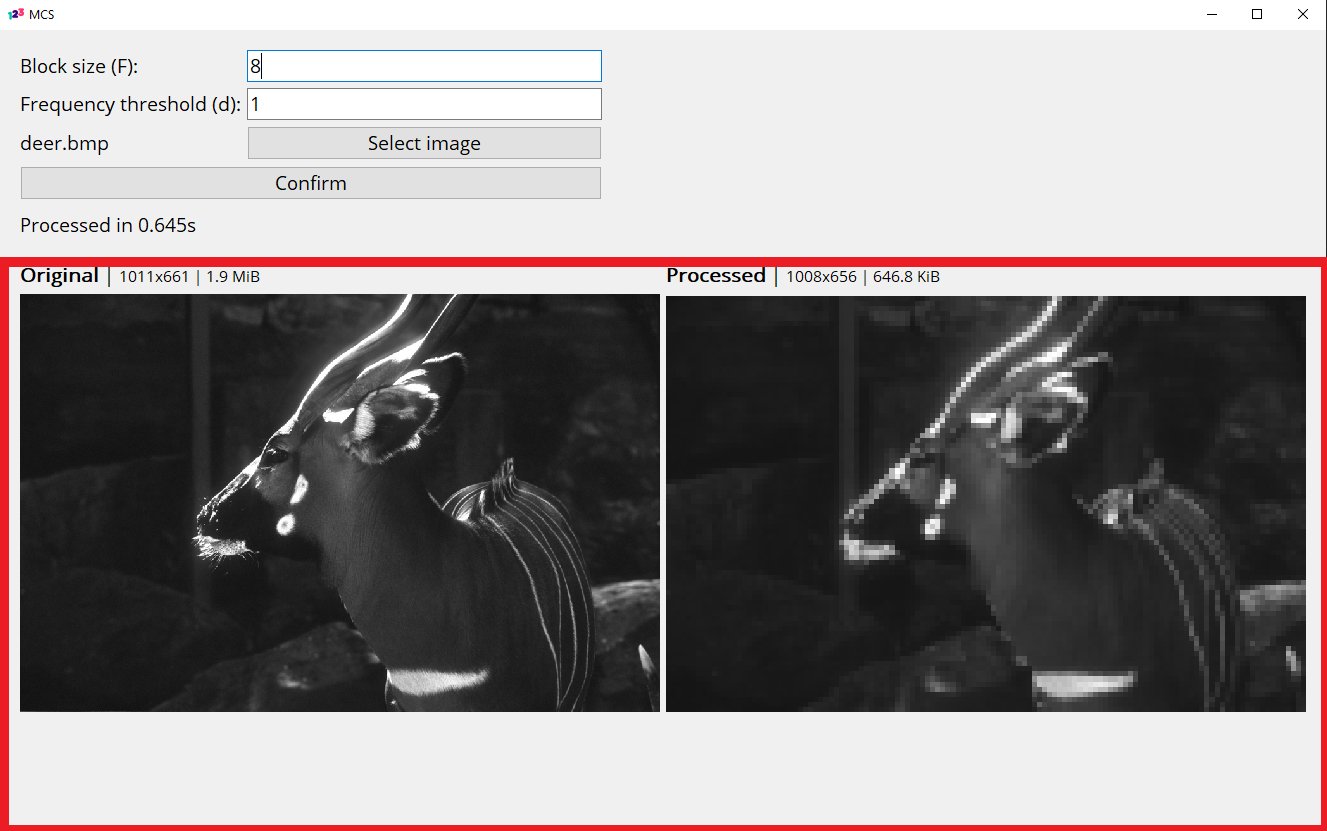
\includegraphics[scale=0.3]{content}\centering
    \caption{Content}\label{fig:content}
\end{figure}